\chapter{Results and evaluation} \label{chap:results}
\section{Accuracy of Iteration 1}
As mentioned in \autoref{ssec:iteration1layers}, various combinations of LSTM layers and Dense layers were tested,
each with various sizes. The results of all of the models can be seen in the \autoref{fig:iteration1_all_accuracy}
The results of the best model can be seen in \autoref{fig:iteration1_best_accuracy}
\subsection{Accuracies of all tests}
\begin{figure}[ht]
    \centering
    \subfloat[\centering Iteration 1 Validation Accuracies]{{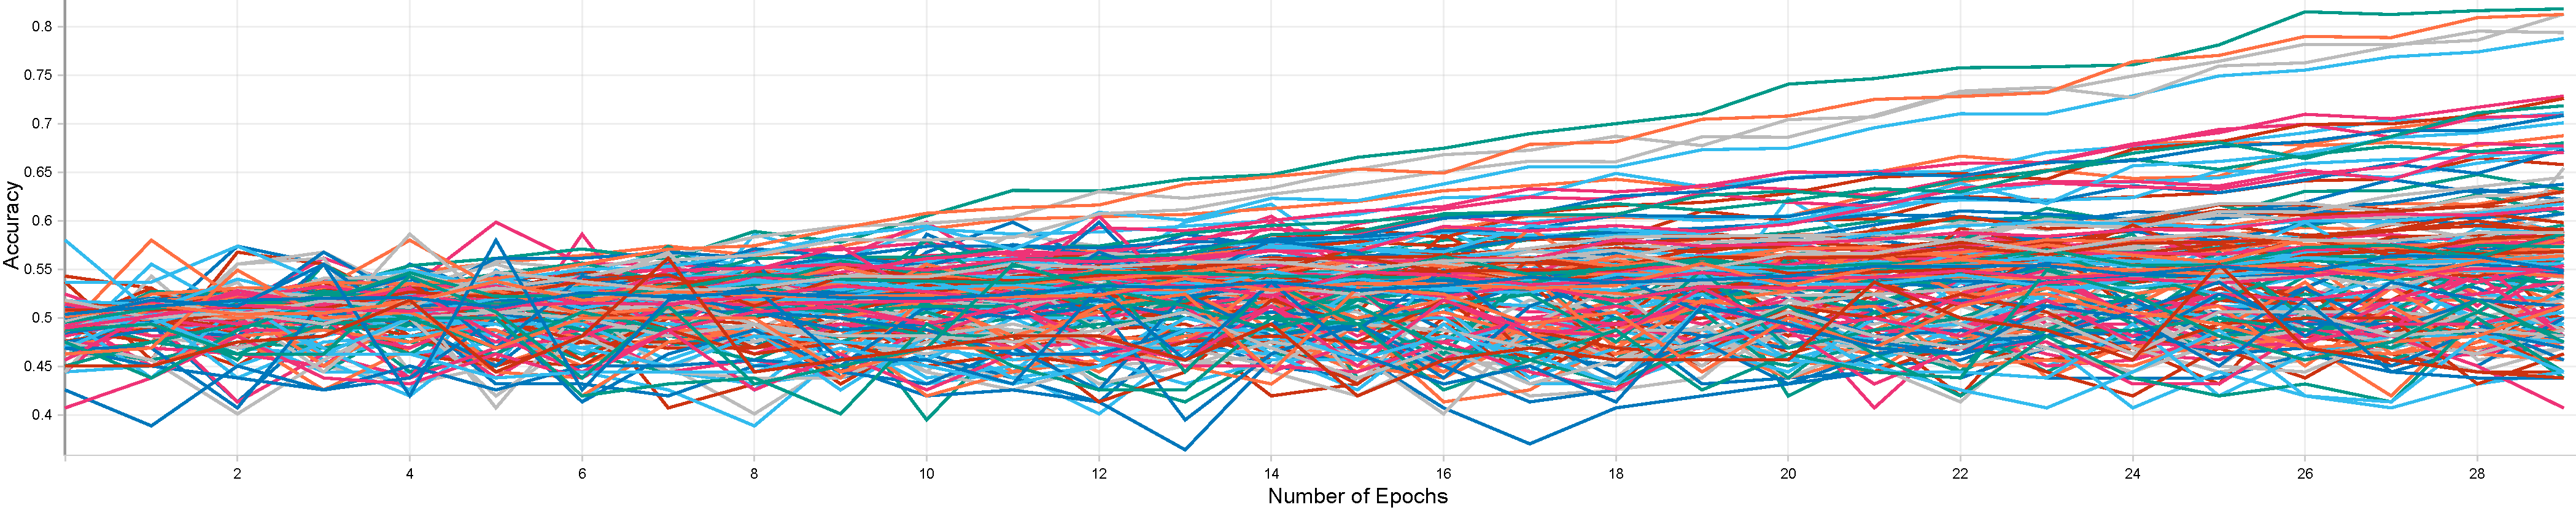
\includegraphics[width=0.45\columnwidth]{figures/results/iteration1_all_accuracy.pdf}}}%
    \qquad
    \subfloat[\centering Iteration 1 Validation Losses]{{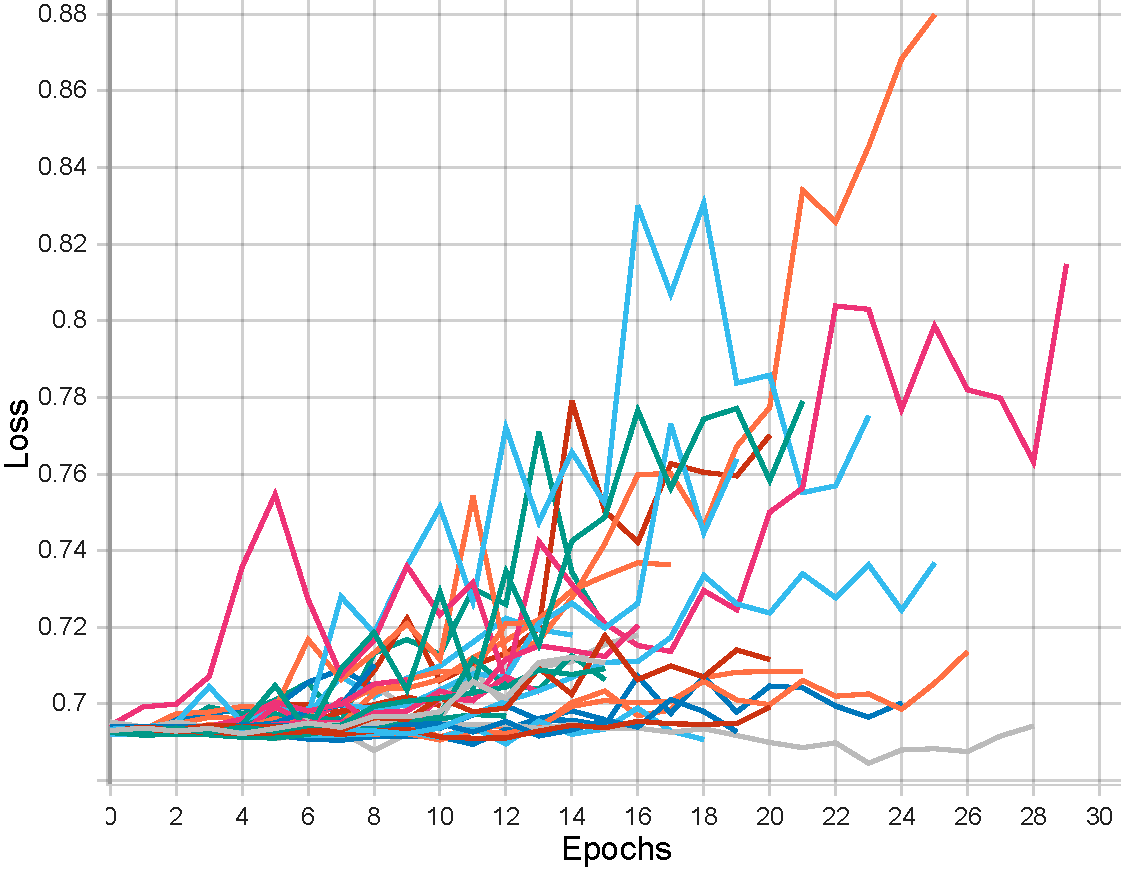
\includegraphics[width=0.45\columnwidth]{figures/results/iteration1_all_loss.pdf}}}%
    
    \caption[Figure of accuracies and losses for Iteration 1]{Figure of all validation accuracies and losses of the combinations of LSTM Layers and Dense Layers}
    \label{fig:iteration1_all_accuracy}
\end{figure}
\FloatBarrier

There are varying degrees of success with different combinations of layers; some do not improve in accuracy and others do.
The validation losses using the sparse categorical loss function as described earlier in \autoref{ssec:iteration1:ai_model}
were used to help identify which models had the lowest error rate; and as an increasing validation
loss is an indicator of overfitting, it was used to filter models showing overfitting.

\subsection{Accuracies of the best result}
\begin{figure}[ht]
    \centering
    \subfloat[\centering Iteration 1 Validation Accuracies]{{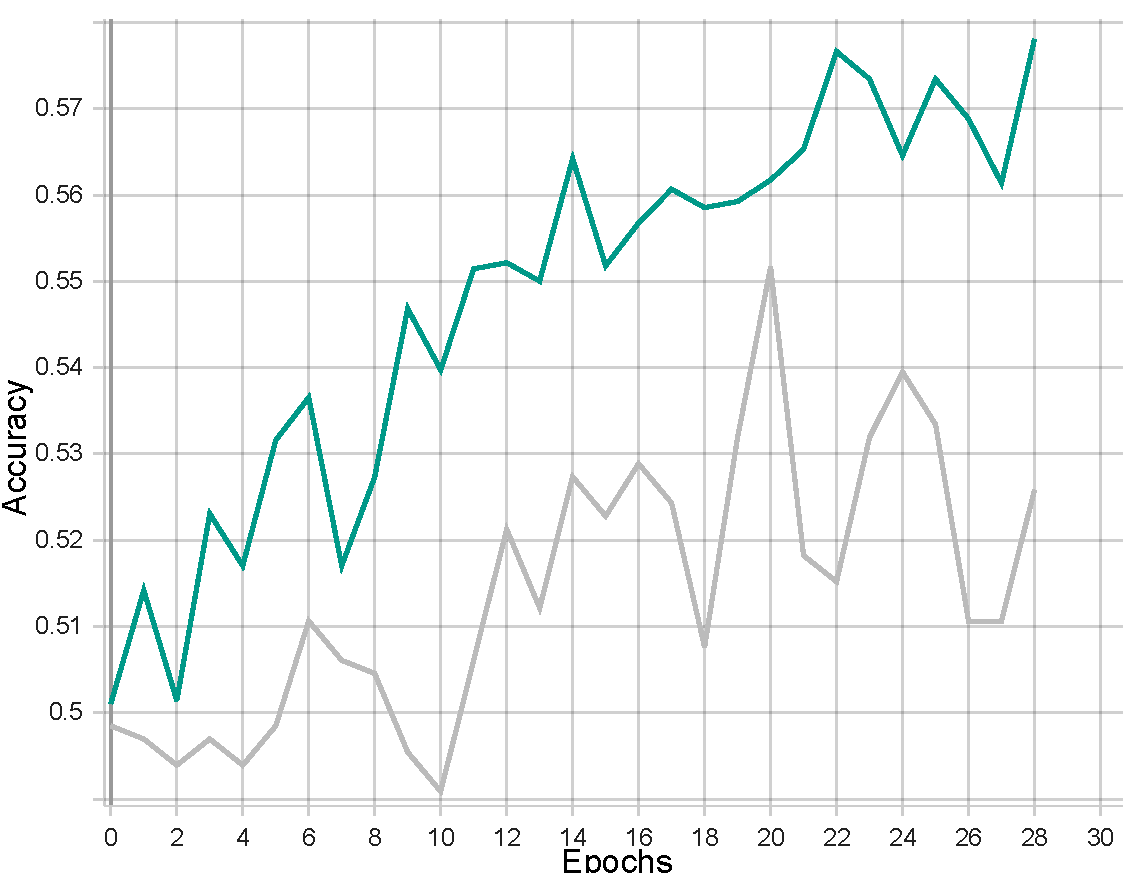
\includegraphics[width=0.45\columnwidth]{figures/results/iteration1_1lstm32_2dense32_accuracy.pdf}}}%
    \qquad
    \subfloat[\centering Iteration 1 Validation Losses]{{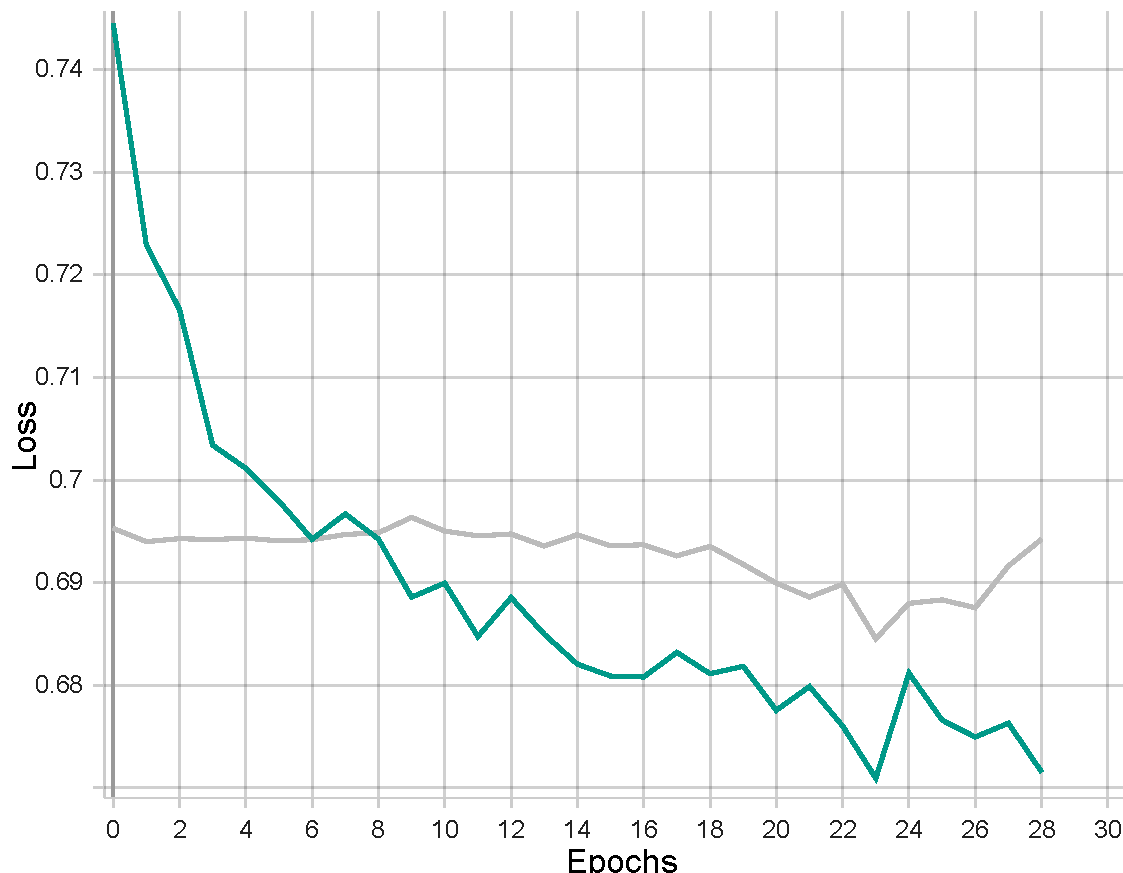
\includegraphics[width=0.45\columnwidth]{figures/results/iteration1_1lstm32_2dense32_loss.pdf}}}%
    \caption[Figure of losses of the best model for Iteration 1]{Figure of losses of the best model of Iteration 1}
    \label{fig:iteration1_best_loss}
\end{figure}
\FloatBarrier
The best model found within this iteration was one with a single LSTM layer of size 32 and a single Dense layer of size 32 followed
by the final Dense layer of size 2. The validation loss shows little overfitting. At 20 epochs, the validation accuracy
reaches its highest value of 55.17\% whilst the training accuracy reached above 56.17\%.
\subsection{Evaluation of iteration 1}
With a validation accuracy above 55\% it suggests that there is improvement above a random choice.
There are various limitations with regards to iteration 1. This iteration does not test various combinations of input features nor does
it test various sequence lengths. Furthermore, it does not yet utilise the CNN + LSTM model, which has been identifed as the optimal model
in the literature review.

\section{Accuracy of Iteration 2}
As mentioned in \autoref{ssec:iteration1layers}, various combinations of LSTM layers and Dense layers were tested,
each with various sizes. The results of all of the models can be seen in the \autoref{fig:iteration1_all_accuracy}
The results of the best model can be seen in \autoref{fig:iteration1_best_accuracy}
\subsection{Accuracies of all tests}
\begin{figure}[ht]
    \centering
    \subfloat[\centering Iteration 2 Validation Accuracies]{{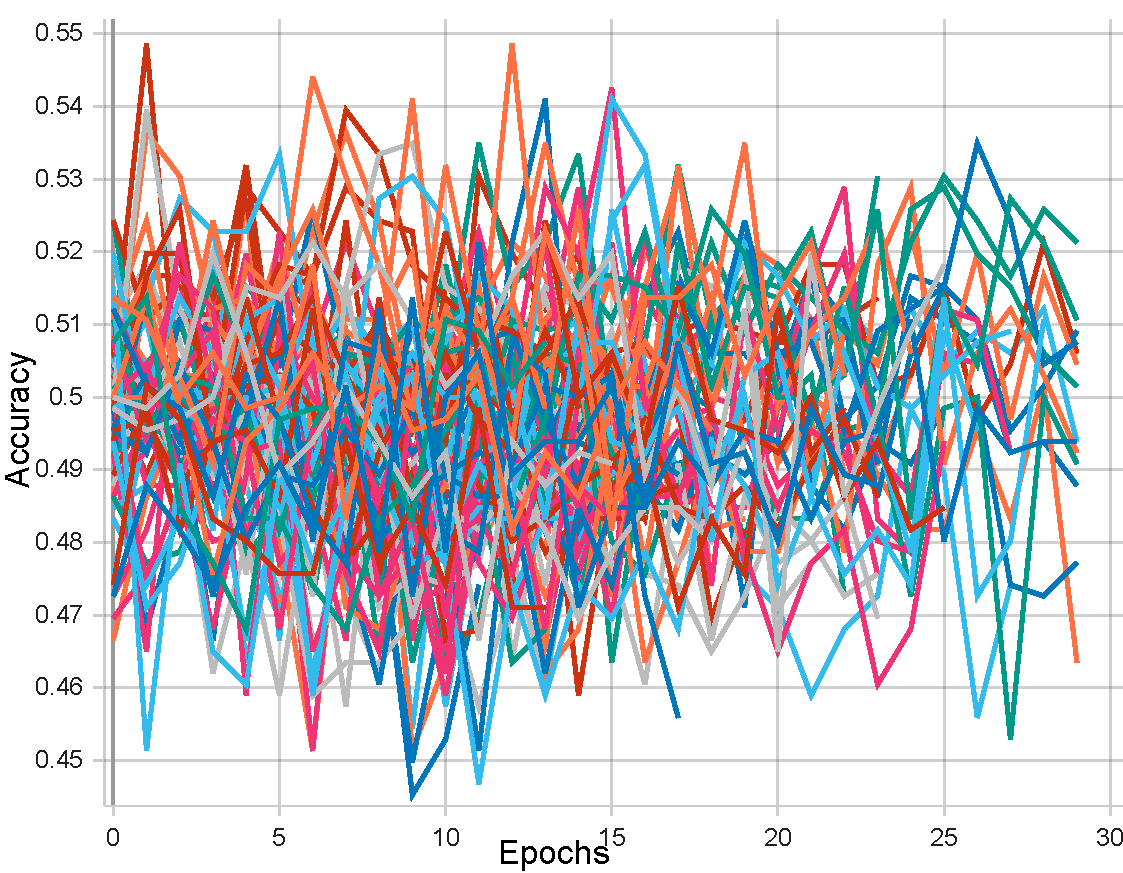
\includegraphics[width=0.45\columnwidth]{figures/results/iteration2_all_accuracy.pdf}}}%
    \qquad
    \subfloat[\centering Iteration 2 Validation Losses]{{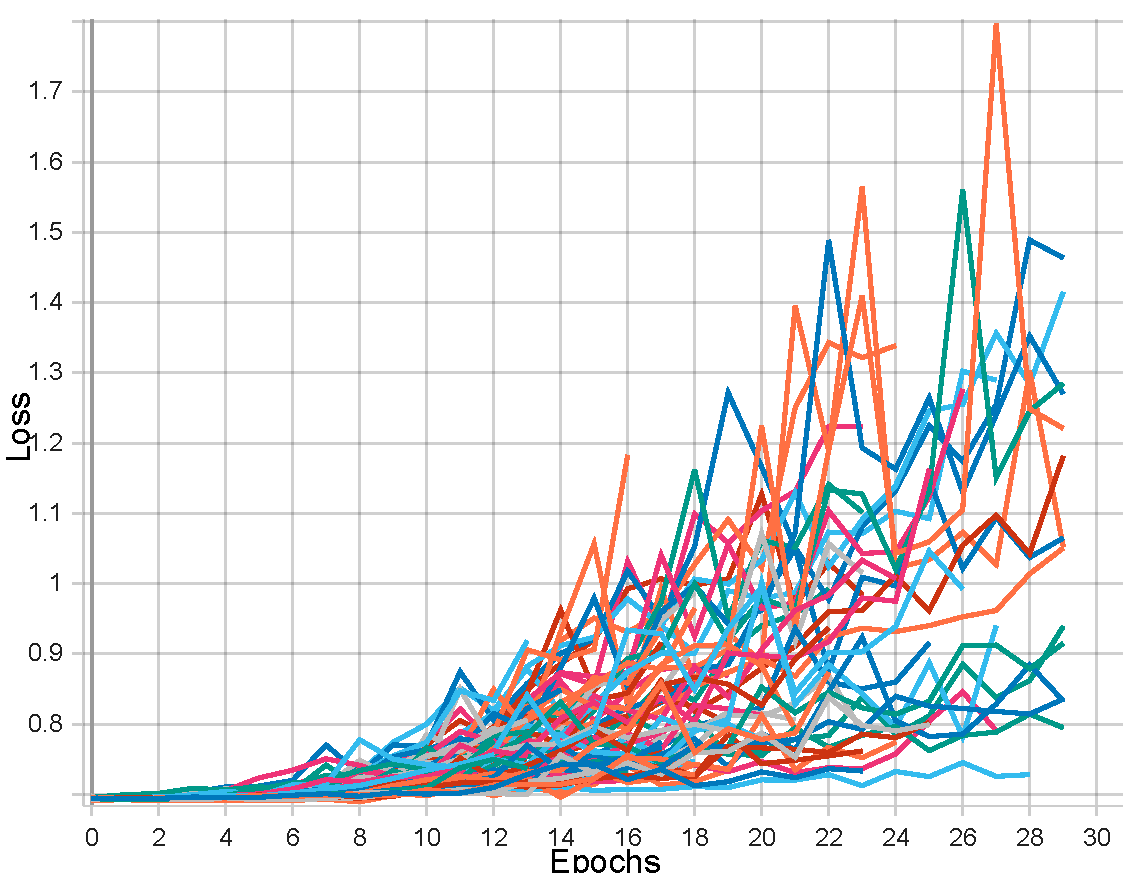
\includegraphics[width=0.45\columnwidth]{figures/results/iteration2_all_loss.pdf}}}%
    
    \caption[Figure of accuracies and losses for Iteration 1]{Figure of all validation accuracies and losses of the combinations of LSTM Layers and Dense Layers}
    \label{fig:iteration1_all_accuracy}
\end{figure}
\FloatBarrier

There are varying degrees of success with different combinations of layers; some do not improve in accuracy and others do.
The validation losses using the sparse categorical loss function as described earlier in \autoref{ssec:iteration1:ai_model}
were used to help identify which models had the lowest error rate; and as an increasing validation
loss is an indicator of overfitting, it was used to filter models showing overfitting.

\subsection{Evaluation of iteration 1}